% LTeX: enabled=false
\documentclass[12pt,oneside]{article}

%%%%%%%%%%%%%%%%%%%%%%%%%%%%
%%   Additional Packages  %%
%%%%%%%%%%%%%%%%%%%%%%%%%%%%
\usepackage{acronym}
\usepackage{enumitem}
\usepackage{a4wide}
\usepackage{fancyhdr}
\usepackage{graphicx}
\usepackage{palatino}
\usepackage{blindtext}
\usepackage{multirow}
\usepackage[ruled,longend]{algorithm2e}
\usepackage{float}
\usepackage{tabularx}

\usepackage[T1]{fontenc}
\usepackage[utf8]{inputenc}

\usepackage{listings}
% Listings configuration: monospaced style, line numbers, line breaks and UTF-8 input
\lstset{
  basicstyle=\ttfamily\small,
  breaklines=true,
  % inputencoding=utf8,
  % Map common German characters so listings shows them correctly under pdflatex
  literate={ä}{{\"a}}1 {ö}{{\"o}}1 {ü}{{\"u}}1 {Ä}{{\"A}}1 {Ö}{{\"O}}1 {Ü}{{\"U}}1 {ß}{{\ss}}1
}

% Links without borders/highlighting
\usepackage[bookmarks, pdfborder={0 0 0}]{hyperref}

\usepackage[justification=centering]{caption}
\usepackage{csquotes}

% APA Style für Bibtex
\usepackage[style=apa,natbib=true,backend=biber]{biblatex}

\DefineBibliographyStrings{english}{
  bibliography = {References},
}
\bibliography{literature}

%%%%%%%%%%%%%%%%%%%%%%%%%%%
%% Definition der Header %%
%%%%%%%%%%%%%%%%%%%%%%%%%%%

\pagestyle{fancy}
\fancyhf{}
\cfoot{\thepage}
\setlength{\headheight}{16pt}

%%%%%%%%%%%%%%%%%%%%%%%%
%% Input of Titlepage %%
%%%%%%%%%%%%%%%%%%%%%%%%
%%%%%%%%%%%%%%%%%%%%%%%%%%%%%%%
%%  Definition of titlepage  %%
%%  Do not edit              %%
%%%%%%%%%%%%%%%%%%%%%%%%%%%%%%%

\newcommand{\UDOTitle}[9]{

  \thispagestyle{empty}
  
\includegraphics[width=3in]{images/tud_logo_rgb.jpg}
  \vspace*{\stretch{1}}
  \\
  {\parindent0cm
  \rule{\linewidth}{.1ex}}
  \begin{flushright}
    \vspace*{\stretch{1}}
    \sffamily\bfseries\Huge
    #1\\
    \vspace*{\stretch{1}}
    \sffamily\bfseries\large
    #2\\
    \vspace*{\stretch{1}}
  \end{flushright}
  \rule{\linewidth}{.1ex}

  \vspace*{\stretch{1}}
  \begin{center}

    \vspace*{\stretch{1}}
    \large #5\\

    \vspace*{\stretch{1}}
    \large Course of Studies: #4 \\[1mm]
    \large Matricle Number: #3\\[1mm]
    \large Supervisor: #8 \\[1mm]
    \large Co-Supervisor:  #9 \\[1mm]

    \vspace*{\stretch{1}}
    \large Time Frame: #6 -- #7

    \vspace*{\stretch{2}}
    \large Chair for Enterprise Computing\\
    \large Faculty for Computer Science\\
  \end{center}
}


%%%%%%%%%%%%%%%%%%%%%%%%%%%%
%% Beginning of Document %%
%%%%%%%%%%%%%%%%%%%%%%%%%%%%

\begin{document}
% Include helper commands
% LTex: enabled=false
\newcommand{\tablespacing}{
    \setlength{\tabcolsep}{12pt}
    \renewcommand{\arraystretch}{1.5}
}

\newenvironment{ctable}[1][ht]{
    \begingroup
    \tablespacing

    % Suppress underfull/overfull box warnings locally inside tables \hbadness controls reporting of underfull hbox
    % badness; setting it % to 10000 suppresses those warnings. \vbadness does the same for vboxes.
    \hbadness=10000
    \vbadness=10000

    \begin{table}[#1]
    \centering
}{
    \end{table}
    \endgroup
}

% LTex: enabled=true


\sloppy

  \UDOTitle
      {Effects of Explainability Alternatives in Generative AI on Users' Cognition and Metacognition}   % Titel der Arbeit
      {Til Goepfert}                                                                                   % Vor- und Nachname des Autors
      {238061}                                                                                          % Matrikelnummer des Autors
      {Master Applied Computer Science}                                                                  % Studiengang
      {Master Thesis}                                                                       % Art der Arbeit
      {30.04.2025}                                                                                      % Tag der Anmeldung
      {30.10.2025}                                                                                      % Tag der Abgabe
      {Prof. Dr. Christian Janiesch}                                                                    % Name des Erstgutachters
      {Dr. Philip Stahmann}                                                                             % Name des Zweitgutachters

  \clearpage

\pagenumbering{Roman}
    \setcounter{page}{1}

\clearpage

%%%%%%%%%%%%%%%%%
%%  Abstract   %%
%%%%%%%%%%%%%%%%%
% \markboth{Abstract}{Abstract}
% \section*{Abstract}
% Zusammenfassung in englischer Sprache.


% \clearpage

\lhead{}

\tableofcontents
\thispagestyle{empty}
\clearpage

\pagenumbering{Roman}
    \setcounter{page}{3}

\addcontentsline{toc}{section}{\listfigurename}
\listoffigures
\clearpage

\addcontentsline{toc}{section}{\listtablename}
\listoftables
\clearpage

\addcontentsline{toc}{section}{Acronyms}
% !TEX root = main.tex

\section*{Acronyms}
% nur bei Bachelor- und Masterthesis

\begin{acronym}[XAI] %Wert in eckiger Klammer ist durch die längste Abkürzung zu substituieren
    \acro{AI}{Artificial Intelligence}

    \acro{COPD}{Chronic Obstructive Pulmonary Disease}
    \acro{CoT}{chain-of-thought}
    \acro{CSE}{Computer Self-Efficacy}

    \acro{EU}{European Union}

    \acro{LLM}{Large Language Model}

    \acro{NASA}{National Aeronautics and Space Administration}
    \acro{NDM}{Naturalistic Decision-Making}

    \acro{STEM}{Science, Technology, Engineering, and Mathematics}

    \acro{TAM}{Technology Acceptance Model}
    \acro{TLX}{Task Load Index}

    \acro{XAI}{Explainable Artificial Intelligence}
\end{acronym}

\clearpage


%%%%%%%%%%%%%%%%
%%  Settings  %%
%%%%%%%%%%%%%%%%
\cleardoublepage
\pagenumbering{arabic}
    \setcounter{page}{1}
\lhead{\nouppercase{\leftmark}}

%%%%%%%%%%%%
%%  Main  %%
%%%%%%%%%%%%

% Chapters with page breaks
\section{Introduction} \label{sec:introduction}

The advent of generative \ac{AI} has sparked unprecedented public interest in \ac{AI} with a wide range of applications, from text generation \parencite{OpenAI2022} to image synthesis \parencite{Rombach2021}. This public interest has driven significant advancements in the field of generative \ac{AI} and widespread adoption across various industries. In particular \acp{LLM} have gained attention due to their versatility and consequently have been widely adopted in the form of chatbots, such as ChatGPT \parencite{OpenAI2025} or Claude \parencite{AnthropicInc2025}. Through advances like reasoning \parencite{OpenAI2024a} and tool use \parencite{AnthropicInc2024} the technical capabilities of \acp{LLM} have outpaced the research on explainability and human-\ac{AI} interaction.

Interpretability is widely recognized as essential for building trust and fostering acceptance of \ac{AI} systems among users \parencite{Arrieta2020,Shin2021}. \ac{XAI} research has provided various methods to explain the outputs of discriminative \ac{AI} systems with LIME \parencite{Ribeiro2016} and SHAP \parencite{Lundberg2017} being two of the most prominent examples. However, these models are not directly applicable to generative \ac{AI}, due to the different nature of their outputs.

With growing adoption of \ac{AI} systems — also in critical domains like healthcare and infrastructure — the need for responsible and effective utilization of \ac{AI} outputs becomes paramount. Some recent works have investigated the cognitive and metacognitive aspects of human-\ac{AI} interaction as well as the perception of \ac{AI} systems, showing the importance of correct handling of \ac{AI} outputs for effective collaboration \parencite{Jussupow2021,Kazemitabaar2024}. However, the effects of explanations on the interaction with generative \ac{AI} systems remain largely unexplored, creating a research gap.

These developments give rise to three key problems that this thesis aims to address:

\begin{enumerate}
    \item Existing explainability techniques are primarily designed for discriminative models and do not adequately address the unique challenges posed by generative models. New methods are needed to provide meaningful explanations for the outputs of generative \ac{AI} systems, that can be understood by lay users.
    \item While some studies have explored the cognition and metacognition of \ac{AI}-assisted decision-making, there is no research on the effects of explanations or cognition and metacognition in the context of generative \ac{AI}.
    \item The studies performed so far have mostly focused on qualitative analysis creating a need for quantitative research to validate findings and provide generalizable insights into human-\ac{AI} interaction with generative models.
\end{enumerate}

These problems are exacerbated by increasing regulation of \ac{AI} systems, such as the \ac{EU} \ac{AI} Act \parencite{EuropeanUnion2024}, which mandates transparency and accountability for almost all \ac{AI} applications. Addressing these challenges is crucial for ensuring that generative \ac{AI} systems are not only powerful but also trustworthy and user-friendly.

\subsection{Research Objectives} \label{subsec:research-objectives}

This thesis aims to contribute to the field of explainable generative \ac{AI} by contributing insights into explainability techniques and their effects on user cognition and metacognition when interacting with generative \ac{AI} systems. Two key research questions guide this work:

\begin{enumerate}[label=(\textbf{RQ\arabic*}),leftmargin=4em]
    \item How does explainable generative \ac{AI} affect problem-solving strategies?
    \item What metacognitive processes do users engage in when using explainable generative \ac{AI} for problem-solving?
\end{enumerate}

To address these questions, this thesis will perform a short literature review of existing explainability techniques, with a focus on their applicability to generative \ac{AI} systems. Additionally, research on cognition and metacognition in human-\ac{AI} interaction will be summarized. Based on the findings, a user study will be designed to qualitatively and quantitatively assess the effects of explanations on user cognition and metacognition when interacting with generative \ac{AI} systems. Based on existing literature the following hypotheses are formulated to be tested in the user study:

\begin{enumerate}[label=(\textbf{H{\arabic*}}),leftmargin=4em]
    \item Users exhibit a heuristic-systematic approach to their interaction with generative \ac{AI} when solving problems collaboratively \parencite{Jussupow2021}.
    \item Providing explanations for the outputs of a model leads to increased acceptance of the system compared to non-explainable systems \parencite{Li2022}.
    \item Users perceive increased self-efficacy over non-explainable \ac{AI} when provided with explanations for the outputs of a model.
    \item Users feel reduced cognitive load and reduced stress when using explainable generative \ac{AI} compared to non-explainable \ac{AI} systems.
\end{enumerate}


\subsection{Thesis Structure} \label{subsec:thesis-structure}

The remainder of this thesis is structured as follows: Section \ref{sec:state_of_research} provides an overview of the current state of research in explainable generative \ac{AI} and cognitive psychology. It summarizes existing explainability techniques and their applicability to generative \ac{AI} systems as well as relevant research from cognitive psychology. In Section \ref{sec:methodology}, the research methodology is outlined, including the design of the user study, the required chatbot, data collection methods, and analysis procedure. The results of the study are presented in Section \ref{sec:results}, followed by a discussion of the findings in Section \ref{sec:discussion}, including implications for future research and practical applications.

\section{State of Research} \label{sec:state_of_research}

Before presenting the methodology of the study in Section \ref{sec:methodology}, this section provides an overview of the state of research relevant to this thesis. It is structured into three main sections: Section \ref{ssec:xai} presents research into \ac{XAI}, Section \ref{ssec:cognitive_psychology} discusses relevant theories and findings from cognitive psychology, and Section \ref{ssec:cognition_ai_users} presents research into how users cognitively process \ac{AI} output in decision support systems and \acp{LLM}.

\subsection{Explainable AI} \label{ssec:xai}

This Section provides an overview of \ac{XAI} by first defining key terminology in Section \ref{sssec:terminology}, which clarifies the distinctions between interpretability, explainability, and transparency as well as the differences between generative and discriminative \ac{AI}. It then discusses the state of research for explainability methods in Section \ref{sssec:explainability_methods}, highlighting both traditional approaches and recent advancements in the field.

\subsubsection{Terminology} \label{sssec:terminology}

While in the field of \ac{XAI} the terms \textit{interpretability} and \textit{explainability} are often used interchangeably, in cognitive psychology they have distinct meanings. \textit{Interpretability} is a broad concept that encompasses various ways to “provide the meaning in understandable terms to a human” \parencite{Arrieta2020}. \textit{Explainability} is one of these modes, that uses an explanation to convey this meaning \parencite{Lipton2016}. \textit{Transparency} is another mode of \textit{interpretability} that conveys meaning by making the inner workings of a model visible to a human \parencite{Arrieta2020}. The limiting factor for \textit{transparency} is the human's ability to understand the inner workings of a model. \textit{Explainability} on the other hand can be applied to any model, regardless of its complexity, by using post-hoc explainability methods \parencite{Arrieta2020}.

The most important distinction for this thesis is between generative and discriminative models. Conceptually generative and discriminative \ac{AI} both use machine learning to learn patterns from data. They are however fundamentally different in their application. Discriminative models learn the decision boundary between two or more classes and are used for classifying data points into these existing classes. Common use cases include anomaly detection \parencite{Edozie2025, Hilal2022}, image classification \parencite{Lu2007}, and sentiment analysis \parencite{Wankhade2022}. Generative models on the other hand learn the underlying distribution of a dataset and can be used to generate new data points that are similar to the training data. Generative models are frequently used for text generation \parencite{Brown2020} or image synthesis \parencite{Rombach2021}.

In the context of \ac{XAI} generative and discriminative models differ in one key aspect: the type and size of output they produce. In an information theoretical sense, discriminative models produce a small amount of information, like a class label that can be expressed in possibly a few dozen bits in extreme cases \parencite{Schneider2024}. Furthermore, the output is often previously known in the form of existing classes. Generative models on the other hand produce a large amount of information, like a paragraph of text or an image, that can be expressed in the order of megabits \parencite{Schneider2024}. Furthermore, the output is often novel and not previously known. This difference in output has implications for explainability methods and how users interact with and perceive these models. Discriminative models can be designed to be inherently interpretable by using simple models like decision trees or linear regression \parencite{Rudin2019}. Alternatively post-hoc explainability methods can be used to explain complex models like deep neural networks \parencite{Ribeiro2016, Lundberg2017}. Generative models on the other hand are often complex and not interpretable by design, which limits the applicability of inherently interpretable models.

\subsubsection{Explainability Methods} \label{sssec:explainability_methods}

Much research in \ac{XAI} has focused on developing explainability methods for discriminative models. These methods can be broadly categorized into two groups: transparency-based methods and post-hoc explainability methods \parencite{Arrieta2020}. Transparency-based methods aim to make the inner workings of a model visible to a human. This can be achieved by using simple models like decision trees or linear regression that are inherently interpretable \parencite{Rudin2019}. Post-hoc explainability methods on the other hand aim to explain the output of a model without making its inner workings visible. This is achieved by highlighting important features in the input data (like LIME \parencite{Ribeiro2016}) or by approximating the model with a simpler interpretable model (like SHAP \parencite{Lundberg2017}). While these methods have proven to be effective in explaining models, both approaches are very technical and are difficult to understand for non-experts \parencite{Martens2025}.

Recently, new explainability approaches have been proposed that seek to remedy these shortcomings. Counterfactual explanations \parencite{Wachter2017} provide explanations by explaining why an alternative output was not chosen. For example in a loan application, a counterfactual explanation could state that if the applicant had a higher income, the loan would have been approved. Another approach are narrative explanations which use natural language to construct a short narrative around SHAP or counterfactual explanations \parencite{Martens2025}. While experts saw little benefit from narrative explanations, non-experts found them significantly more useful and easier to understand \parencite{Martens2025}.

A third approach involves \ac{CoT} explanations \parencite{Wei2022}, where \acp{LLM} generate intermediate reasoning steps that lead to the final output. These steps can enhance users' perception of transparency by allowing them to follow the model's reasoning process. Moreover, decomposing complex problems into smaller steps has been shown to improve the effectiveness of \acp{LLM} in problem-solving \parencite{Wei2022}. Notably, this technique can be applied to existing models without retraining, as demonstrated in this study. However, it is important to recognize that these intermediate steps are generated by the model itself and may be unfaithful or incorrect \parencite{Turpin2023, Schneider2024}. In a related line of research, \textcite{Lindsey2025} demonstrated that it is possible to identify and visualize specific neurons representing concepts, and to observe activation patterns that resemble a thought process.


\subsection{Cognitive Psychology} \label{ssec:cognitive_psychology}

This Section provides an overview of relevant theories and findings from cognitive psychology. To establish a framework for understanding human cognition, Section \ref{sssec:dual_process} discusses dual process theory. Sections \ref{sssec:heuristics} and \ref{sssec:metacognition} discuss heuristics and metacognition to further elaborate on cognitive processes relevant to this thesis. Finally, Section \ref{sssec:cognitive_offloading} discusses cognitive offloading as this behaviour and its drivers are particularly relevant to human-AI interaction.

\subsubsection{Dual Process Theory} \label{sssec:dual_process}

Dual process theory refers to a group of theories in cognitive psychology that proposes humans have two distinct types of cognitive processing: Type 1 and Type 2 \parencite{Evans2013}. Type 1 processing is intuitive, autonomous processing and often referred to as “System 1” \parencite{Kahneman2011}. Type 2 processing (also “System 2”) on the other hand is deliberate, controlled processing that requires cognitive effort \parencite{Evans2013}. It is often associated with higher-order cognitive functions like reasoning, problem-solving, and decision-making \parencite{Kahneman2011}. Different theories propose different characteristics for both types of processing, but they agree on several core characteristics as summarized in Table \ref{tab:dual_process_characteristics}. The first two rows contain characteristics that are widely agreed upon, while the remaining rows contain characteristics, that find support in some theories, but are not as universally accepted \parencite{Evans2013}.

\begin{ctable}
    \begin{tabular}{l|l}
        \textbf{Type 1} & \textbf{Type 2} \\
        \hline
        Autonomous & Deliberate \\
        Intuitive & Controlled \\
        \hline
        Fast & Slow \\
        Parallel & Serial \\
        Non-conscious & Conscious \\
        Biased responses & Normative responses \\
        Contextualized & Abstract \\
    \end{tabular}
    \caption[Type 1 and Type 2 Characteristics]{Common characteristics of Type 1 and Type 2 processing in dual process theories \parencite{Evans2013}}
    \label{tab:dual_process_characteristics}
\end{ctable}

Different theories propose different relationships between Type 1 and Type 2 processing. Some theories propose a competitive relationship, where both types of processing work in parallel and resolve conflicts if they occur. However, this conflicts with the fact that the two systems are associated with different speeds. If Type 1 processing is faster, conflict resolution would always have to wait for Type 2 processing to finish. Alternatively, a wide range of theories proposes a default-interventionist relationship, where Type 1 processing is the default mode of processing and Type 2 processing only intervenes when necessary \parencite{Evans2013}. There is evidence for both relationships, even attempts to reconcile both relationships into a single theory, but the exact relationship remains an open question \parencite{Evans2013, Djulbegovic2012}. Recent research in the context of \ac{XAI} has interpreted results assuming the default-interventionist relationship is the more accurate one \parencite{Jussupow2021, Shin2021}.

\subsubsection{Heuristics} \label{sssec:heuristics}

Heuristics are methods for problem-solving that use practical and efficient approaches to produce solutions that are not guaranteed to be optimal, but can be achieved much quicker \parencite{Gigerenzer2011}. Heuristics are often contrasted with algorithms, which are systematic and exhaustive methods that guarantee an optimal solution. The research into heuristics goes back on the work of \cite{Simon1955}, who observed that humans often make decisions with limited time, information, and cognitive resources. This results in a behaviour he coined as “satisficing” as a portmanteau of “satisfy” and “suffice” \parencite{Simon1956}. It seeks to describe the behaviour of accepting the first satisfactory solution instead of searching for the optimal one.

Building on this work, \textcite{Tversky1974} identified three key heuristics that humans use in decision-making:

\begin{itemize}
    \item The \textit{Availability} heuristic serves to estimate the likelihood of an event based on how easily examples come to mind. For example, if a person has recently heard about a plane crash, they might overestimate the risk of flying.
    \item \textit{Representativeness} is used to judge the probability of an event based on how similar it is to a prototype. For example, if a person sees someone who is tall and athletic, they might assume that they are a basketball player.
    \item \textit{Anchoring and Adjustment} describe a related set of behaviours where people rely heavily on an initial piece of information (the anchor) when making decisions. For example, if a person is negotiating a salary, they might start with a high anchor and then adjust it downwards.
\end{itemize}

Due to their nature of leaving out information and relying on cognitive shortcuts, heuristics can lead to systematic biases and erroneous decisions. They are also related to dual process theory, as they are often associated with Type 1 processing \parencite{Evans2013}.

\subsubsection{Metacognition} \label{sssec:metacognition}

Metacognition refers to the awareness and understanding of one's own cognitive processes \parencite{Flavell1979}. It involves the ability to monitor, regulate, and control one's own thinking and learning. Metacognition is often divided into two components: metacognitive knowledge and metacognitive regulation \parencite{Schraw2006}. Metacognitive knowledge refers to the knowledge about one's own cognitive processes, including knowledge about strategies for learning and problem-solving. Metacognitive regulation refers to the ability to monitor and control one's own cognitive processes, including planning, monitoring, and evaluating one's own learning and problem-solving activities \parencite{Cross1988}.

Metacognition plays a crucial role in problem-solving, as it allows individuals to reflect on their own thinking and adjust their strategies accordingly. It is also related to heuristics, as metacognition is crucial for correct the application of heuristics and the aversion of biases \parencite{Koriat2010}. In the context of \ac{XAI}, metacognition is relevant because it can influence how users interact with and perceive AI systems. Depending on their metacognitive evaluation of an interaction, users might adjust their reliance on the system. For example, if a user perceives an AI system as reliable and trustworthy, they might rely on it more heavily. Conversely, if a user perceives an AI system as unreliable or untrustworthy, they might be more cautious in their interactions with it \parencite{Jussupow2021, Shin2021}.

\subsubsection{Cognitive Offloading} \label{sssec:cognitive_offloading}

Cognitive offloading refers to the manipulation of one's body or the environment to support cognitive tasks. Examples of cognitive offloading include writing down a shopping list to remember items or tilting one's head to view a rotated image. Cognitive offloading allows individuals “to flexibly deploy ad-hoc mixtures of internal and external processes”, which enables the improvement of cognitive capabilities \parencite{Risko2016}. By offloading cognitive tasks to the environment, individuals can reduce their cognitive demand and free up cognitive resources for other tasks \parencite{Risko2016}.

The propensity to offload cognition is influenced by the internal cognitive demands that would otherwise be necessary \parencite{Gilbert2015, Risko2015}. The evaluation of these cognitive demands are performed as a metacognitive evaluation process. The offloading decision is influenced by a number of factors that are subject to these metacognitive evaluations:

\begin{itemize}
    \item The estimated \textit{cognitive demand} required for the task plays an important role in the decision to offload \parencite{Risko2015}. If the estimated effort is high, individuals are more likely to offload the task to the environment.
    \item The perceived \textit{effort of offloading} is also a crucial factor \parencite{Risko2015}. If the perceived effort is low, individuals are more likely to offload the task.
    \item The decision to offload is also influenced by personal \textit{experiences with offloading} \parencite{Ward2013}. Repeated successful offloading may lead to an inflated perception of one's cognitive capabilities, which can influence future offloading decisions.
\end{itemize}

Like other metacognitive processes, individuals are not always aware of the evaluation process that leads to a cognitive offloading decision \parencite{Schunn2001}. Increased awareness of the decision process can lead to improved strategy selection, but like other metacognitive processes it is subject to biases and errors, which can lead to suboptimal offloading decisions \parencite{Risko2015}. This is particularly relevant in the context of decision support systems, where users might offload cognitive tasks to a system while overestimating its capabilities \parencite{Jussupow2021}. However, humans also show the capability to adapt their cognitive offloading behaviour based on the goals they are trying to achieve \parencite{Weis2019}. If offloading behaviour is considered during system design, systems can be designed to guide users towards beneficial offloading behaviour.

\subsection{Cognition of AI Users} \label{ssec:cognition_ai_users}

Recent research has begun to investigate how users cognitively process \ac{AI} output in decision support systems and \acp{LLM}. Since the field has only recently gained attention, the Section focuses on two recent studies in Section \ref{sssec:studies_ai_cognition}. It then discusses the psychology of explanations in Section \ref{sssec:psychology_explanations} and AI anthropomorphism in Section \ref{sssec:ai_anthropomorphism}.

\subsubsection{Recent Studies on AI User Cognition} \label{sssec:studies_ai_cognition}

Two recent studies have investigated how users cognitively process AI output in decision support systems and \acp{LLM}. Results suggest a heuristic-systematic approach to processing AI output, suggesting that users employ both Type 1 and Type 2 processing when interacting with AI systems \parencite{Jussupow2021,Kazemitabaar2024}. Findings from both studies indicate also that problems arise when users fail to switch from heuristic to systematic processing when necessary.

\cite{Jussupow2021} investigated the cognitive and metacognitive processes of doctors using \ac{AI}-based decision support systems. Their findings present a process model based on \ac{NDM}, where the user initially constructs a \textit{frame} for a decision based on their initial (heuristic) assessment of the situation \parencite{Klein2008, Klein2015}. If the \ac{AI} confirms the frame, users usually accept the frame as final decision. If the \ac{AI} contradicts the frame however, users enter a \textit{belief conflict}, in which they have to decide whether they believe more in their own abilities or the \ac{AI}'s capabilities. “If neither belief is dominant, physicians move into the validation conflict, in which they use additional data to validate their own frame and the AI advice” \parencite{Jussupow2021}. During this conflict, users engage in systematic processing of additional information to find support for either their own decision or the \ac{AI}'s. Failure to correctly switch to systematic processing leads to errors more frequently. The complete process model is shown in Figure \ref{fig:jussupow_process_model}.

\begin{figure}[ht]
    \centering
    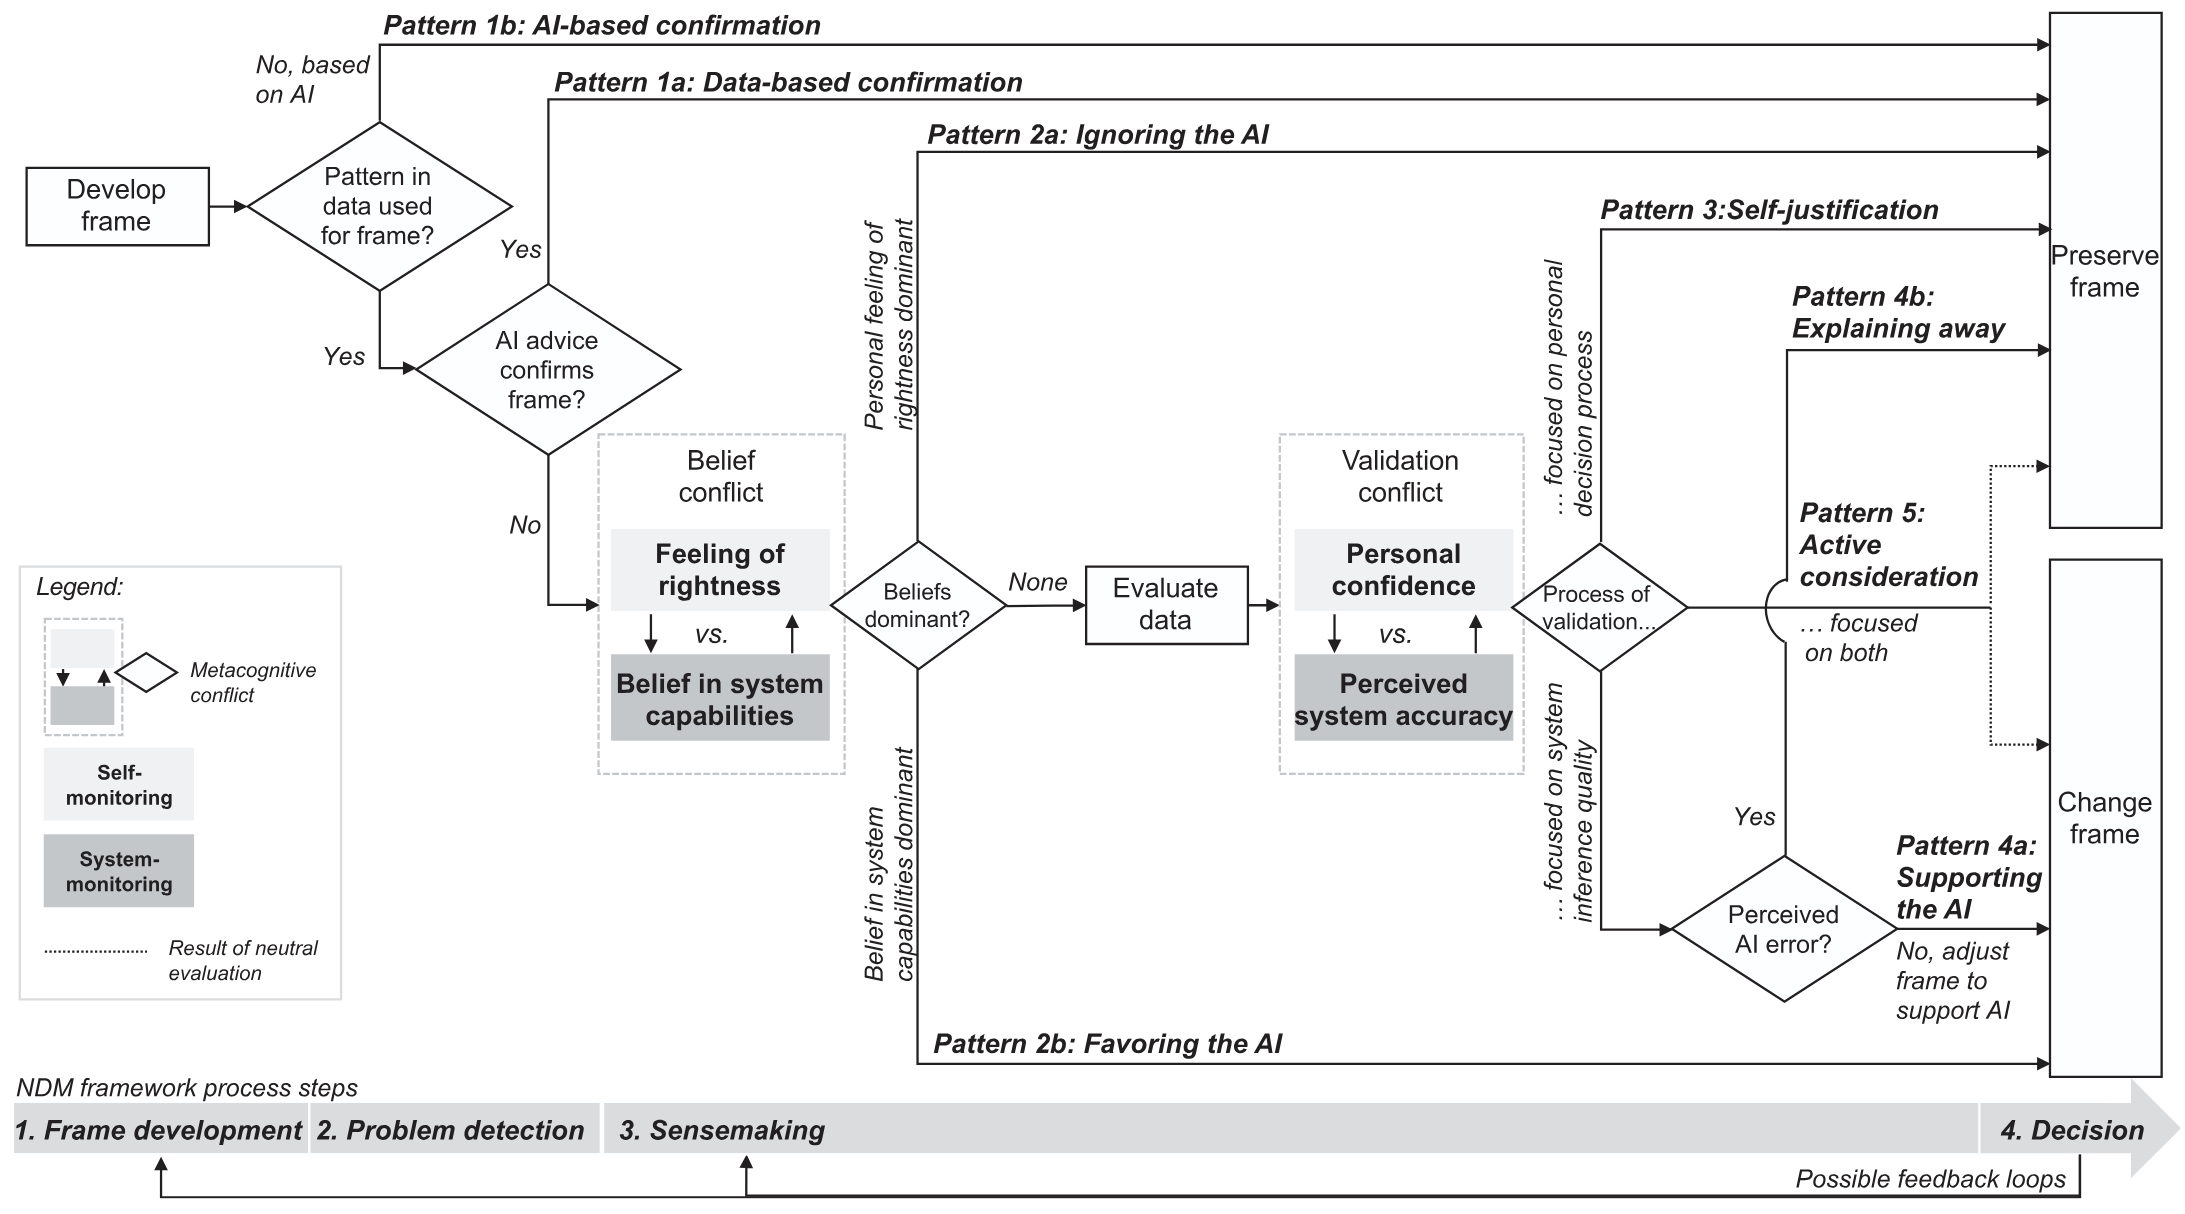
\includegraphics[width=0.8\textwidth]{images/fig_jussupow_model.png}
    \caption[Process Model of AI-Assisted Decision-Making]{Process Model of AI-Assisted Decision-Making \parencite{Jussupow2021}}
    \label{fig:jussupow_process_model}
\end{figure}

In an experiment where researchers performed data analysis tasks with the support of a \ac{LLM}, \cite{Kazemitabaar2024} found that stepwise task decomposition improves the perceived ease of use of the \ac{AI} and reduced frustration. Users cited improved steering and transparency as key factors for this improvement. Additionally, users reported that the ability to have side conversations with the \ac{LLM} to clarify steps or request additional information was particularly important. Furthermore, users found it easier to verify the output and to intervene and fix errors with stepwise decomposition. These findings suggest, that a \ac{CoT} approach can facilitate an improved perception of transparency and act as an explanation for the \ac{LLM}'s output. This improved perception can facilitate the switch from heuristic to systematic processing when necessary, leading to improved decision-making with \acp{LLM}.

\subsubsection{Psychology of Explanations} \label{sssec:psychology_explanations}

\cite{Miller2019} reviewed literature from cognitive psychology and social sciences to identify key challenges for \ac{XAI}. A key finding of the review is that explanations can be seen through three different lenses:

\begin{itemize}
    \item Explanations are a \textit{cognitive process}, that involves the selection and organization of information to create an explanation.
    \item The cognitive process results in a \textit{product}, which is the explanation itself.
    \item Explanations are a \textit{social process}, that involves the interaction between the explainer and the explainee.
\end{itemize}

As discussed in Section \ref{sssec:explainability_methods}, much research has been performed into the \textit{cognitive process} (i.e., generation) and the \textit{product} of explanations. However, the \textit{social process} of explanations has been largely neglected in \ac{XAI} research. \cite{Martens2025} proposed narrative explanations as a way to improve the \textit{social process} of explanations by making them more natural and easier to understand for non-experts. \acp{LLM} offer an additional opportunity to improve the explanation process by enabling interactive explanations through natural language conversations. This allows the \ac{LLM} as the explainer to adapt explanations to the specific needs of the explainee and consequently improve the explanation selection.

Since \cite{Miller2019} published these findings \cite{Wachter2017} proposed counterfactual explanations as a way to improve the effectiveness of explanations. Counterfactual explanations align well with the findings of \cite{Lipton1990}, who identified that humans often do not seek a complete causal explanation, but rather focus on contrasting the event $P$ that occurred with an event $Q$ that did not occur. By focusing on the differences between $P$ (called \textit{fact}) and $Q$ (called \textit{foil}), humans can more easily understand the causal relationships that led to the event. In absence of a clear \textit{foil}, it has to be inferred from context, which emphasizes the importance of explanations being tailored to the explainee.

\subsubsection{AI Anthropomorphism} \label{sssec:ai_anthropomorphism}

Anthropomorphism refers to different facets of the attribution of human characteristics to non-human agents \parencite{Li2022}. In the context of this thesis, the focus lies on the perception of \ac{AI} systems as human-like. This attribution of human-like characteristics can significantly influence how users perceive and therefore interact with the system \parencite{Li2022}. Primarily, anthropomorphism influences users' trust in the system \parencite{Shin2021}. It also influences users acceptance and intention to use the system \parencite{Li2022}. Given these findings, it can be assumed that anthropomorphism acts as a moderating variable, that could reduce users criticality towards \ac{AI} and hinder effective switching from heuristic to systematic processing when necessary.

% TODO: find more to say here?

\section{Methodology} \label{sec:methodology}

\subsection{Research Design} \label{ssec:research_design}

\subsection{Study Execution} \label{ssec:study_execution}

\subsection{Data Analysis} \label{ssec:data_analysis}

\section{Results} \label{sec:results}

The following section presents the findings of the study. The results are organized into qualitative results in section \ref{ssec:qual_results} and quantitative results in section \ref{ssec:quant_results}. Before presenting the results, the characteristics of the study participants are shortly described in section \ref{ssec:study_participants}.

\subsection{Study Participants} \label{ssec:study_participants}

Study participants were recruited through two channels: (1) students associated with the university chair for Enterprise Computing and (2) colleagues of the author. A total of 15 participants was recruited throughout July 2025. With 13 of the participants the experiment was conducted in August 2025, while 2 participants dropped out of the study due to time constraints. One participant was excluded from the analysis due to not following the instructions for the think aloud protocols sufficiently, producing unusable data. The final sample thus consists of 12 participants.

The participants were exclusively male, with additional demographic information presented in Table \ref{tab:age_dist} and Table \ref{tab:edu_bg}. The final sample consisted of 12 participants, with 5 in group (B) without explanations and 7 in group (E) with explanations.

\begingroup
\tablespacing

\begin{table}[ht]
    \parbox{.45\linewidth}{
        \centering
        \begin{tabular}{cc}
            Age Range & Count \\
            \hline
            20--29 & 8 \\
            30--39 & 2 \\
            40--49 & 1 \\
            60--69 & 1
        \end{tabular}
        \caption{Age Distribution of Participants}
        \label{tab:age_dist}
    }
    \hfill
    \parbox{.45\linewidth}{
        \begin{tabular}{cc}
            Education Level & Count \\
            \hline
            University Degree & 8 \\
            Vocational Training & 2 \\
            Grammar School & 2
        \end{tabular}
        \caption{Educational Background of Participants}
        \label{tab:edu_bg}
    }
\end{table}

\endgroup

\subsection{Qualitative Results} \label{ssec:qual_results}

The qualitative data collected from the think-aloud protocols was analysed through two rounds of coding as described in section \ref{sssec:qualitative_analysis}. The codes produced in the first round of coding, were then grouped into categories (axes). Overall four conclusions are drawn from the qualitative data, which are presented in the following.

\subsubsection{Usage Patterns} \label{sssec:usage_patterns}

Participants in both groups utilized the chatbot for varying purposes, if they decided to use it at all. Questions posed to the chatbot ranged from very specific questions for formulas to more general questions asking for a solution approach. Some participants used the chatbot to verify their own solutions or solution approaches. Taking into account the possibility of non-use of the chatbot, four different usage patterns can be identified:

\begin{ctable}
    \begin{tabularx}{\textwidth}{l|X|X}
        \textbf{Usage Pattern} & \textbf{Definition} & \textbf{Example} \\
        \hline
        Non-Use & The participant does not use the chatbot at all & “I did not need the LLM for that.” (P3) \\
        Fact Questions & The participant uses the chatbot to ask for specific facts, formulas, or definitions & “What is the formula for the circumference of a circle if 'r' is given?” (P13) \\
        Approach Questions & The participant uses the chatbot to ask for a solution or solution approach & “What approach should I take and how should I take the relationship into account.” \\
        Validation Questions & The participant uses the chatbot to verify their own solution or solution approach & “I'll send the solution to [\dots] the chatbot to see if it makes sense.” (P5)
    \end{tabularx}
    \caption{Usage Patterns of the Chatbot}
    \label{tab:usage_patterns}
\end{ctable}

The usage pattern of \textit{Non-Use} is noteworthy, as the decision to not use the chatbot was only commented by two participants (P3, P8) after the fact. Other participants also solved tasks without using the chatbot, but did not mention this decision at all. This indicates that the decision whether to use the chatbot or not, is not a conscious decision, but rather a subconscious one. Additionally, the usage patterns could change during the same task, with participants starting with approach questions (for an initial hint) and later switching to validation questions, indicating that the a (subconscious) decision is made for each interaction with the chatbot.

Overall the usage patterns align with the behaviour for cognitive offloading described in section \ref{sssec:cognitive_offloading}. This particularly applies to the decision whether and how to use the chatbot, which is “[\dots] influenced by a metacognitive evaluation of the available options” \parencite{Risko2015}. A factor that could influence these decisions is the perceived difficulty of the task, which was mentioned by several participants prior to using the chatbot (P1, P5). Based on the behaviour of participants combined with the think-aloud protocols, it can also be assumed, that the \textit{Availability} heuristic \parencite{Tversky1974} played a role in the decision whether to use the chatbot or not. Participants more often used the chatbot for developing a solution approach, if they had exhausted their own ideas (P3, P8, P10). A third factor that could influence is the perceived effort of using the chatbot compared to solving the task without it. This is supported by the fact that some participants justified their use of the chatbot by stating they did not “want to [solve the problem]” themselves (P5).

\subsubsection{Errors and Conflicts} \label{sssec:errors_conflicts}

Participants in both groups encountered errors and conflicts during their interactions with the chatbot. It is important to note, that the problems described here, are conflicts and errors perceived by the participants, and not objective conflicts. These perceived issues can be grouped into three categories, which are presented in Table \ref{tab:conflicts_errors}.

% ToDo: Is distinguishing between misundersanding and incorrect information necessary sensible?
% - since the issues are distinguished by the participants, it is irrelevant whether the information is actually incorrect or not

\begin{ctable}
    \begin{tabularx}{\textwidth}{l|X|X}
        \textbf{Category} & \textbf{Definition} & \textbf{Example} \\
        \hline
        Incorrect Information & The chatbot provides factually incorrect information & “But it [the chatbot] says, that I have $\overline{AB}$ given, which is not correct either.” (P4) \\
        Misunderstanding & The participant misinterprets the chatbot's response & “Okay, 'intersects at two points' is the same as 'touches at two points'. Not for me.” (P11) \\
        Conflicting Information & The chatbot provides information that contradicts previous responses or known facts & “First it [the chatbot] says 'almost correct', then 'correct' [for the same solution]” (P11) \\
    \end{tabularx}
    \caption{Categories of Errors and Conflicts with the Chatbot}
    \label{tab:conflicts_errors}
\end{ctable}

The most frequently encountered issue was \textit{Incorrect Information}, where participants perceived the chatbot's responses as factually incorrect (P4, P8, P13, P15). In many cases however, the participants simply misread the response (P8) or forgot information provided in the task or previously calculated (P4, P13, P15). Similarly, \textit{Misunderstandings} were often due to participants misreading or misinterpreting the chatbot's response (e.g. P11, P13). Conversely, during task 54 participants frequently received wrong advice from the chatbot, but did not recognize the error immediately. Given that none mentioned the wrong information from the chatbot in their think-aloud protocols, it can be assumed, that a form of “satisficing” \parencite{Simon1955} took place, where participants accepted the chatbot's response without further scrutiny.

The conflict behaviour observed during the study aligns with the findings from \cite{Jussupow2021}, where medical practitioners experienced similar conflicts when using a decision support system to diagnose \ac{COPD}. When being confronted with AI decisions that conflicted with their own assessment, the practitioners experience a \textit{belief conflict}, where they had to decide whether to trust their own judgement or the AI's decision. A similar conflict was observed in this study, but participants did rarely verbalize the conflict. Instead, most participants moved to the \textit{validation conflict}, seeking additional information to resolve the conflict. “Aiming to resolve the validation conflict, decision makers continuously evaluate their personal confidence into their own frame against their perception of the system accuracy” \parencite{Jussupow2021}. During the study the validation conflict was often resolved users discovering their own mistakes (P4, P9, P15) and adopting the chatbot's position.

\subsubsection{Reflection and Learning}

The think-aloud protocols also showed, that participants did not actively reflect on every interaction with the chatbot. Reflection primarily occurred after participants resolved a conflict with the chatbot (P8, P11) or when they were positively surprised by the chatbot's assistance (P1, P2). Participant 8 noted that it “sad, that the chatbot does not detect these logic errors” after realizing he had made a mistake transforming a formula step by step. On the other hand, participant 1 assessed, that “the chatbot helped quite a lot”. It is unclear under which conditions participants actively reflect on interaction with the chatbot, but several general cognitive patterns may play a role:

\begin{itemize}
    \item \textbf{Abnormality:} % Arrieta2020? Miller2019?
    \item \textbf{Anchoring \& Ajdustment:} % Tversky1974
    \item \textbf{Confirmation Bias:} % Nickerson1998
\end{itemize}

Since questionnaires were only administered after all tasks were completed, it is unclear whether participants' perceptions of the chatbot changed during the study.

\subsubsection{Additional Observations} \label{sssec:additional_observations}

Participants rarely actively engaged with the explanations provided by the chatbot in group (E). Only two participants (P8, P9) explicitly mention the \ac{CoT} explanation. In both instances the explanation was treated as additional information, that was used once the user was stuck. Other participants in group (E) did not mention the explanations at all. Similarly, users in group (B) did not comment on the lack of explanations. Therefore, the explanations did not seem to have a significant impact on the participants' behaviour or perception of the chatbot. The instances where the explanations were used, could also be due to the interface design, which initially hid the explanations in a collapsed section.

\subsection{Quantitative Results} \label{ssec:quant_results}

\section{Discussion} \label{sec:discussion}

The discussion section of this thesis will be split into three main parts: A summary of the main findings and the implications for the hypotheses and research questions posed in the introduction are presented in Section~\ref{ssec:summary}. Section \ref{ssec:implications} discusses the implications of these findings and suggests avenues for future research building on this work. Finally, Section \ref{ssec:limitations} addresses the limitations of the current study and how they might be mitigated in future work.

\subsection{Summary of Findings} \label{ssec:summary}

This thesis investigates the cognitions and metacognitions of \ac{LLM} users in problem-solving tasks and the effect explanations have on these processes. Current research primarily focuses on methods for generating explanations, that are understandable to lay users, and their effects on task performance. This study sought to investigate how the underlying cognitive and metacognitive processes are affected by explanations.

Firstly, the study finds that problem solvers using \acp{LLM} exhibit a range of collaboration strategies, where the role of the \ac{LLM} can vary from an interactive knowledge base to a collaborative partner. The choice of strategy is influenced by task-dependent factors, such as the complexity of the problem, the user's perception of their own expertise, and the perceived capabilities of the system. The decision for a given strategy is subconscious, likely based on heuristic assessments of the aforementioned factors. Users can also change their strategy dynamically based on their evolving perceptions of the task and the model's performance. This suggests an ongoing evaluation of the interaction with the \ac{LLM}. Explanations have no effect on the choice of collaboration strategy.

Secondly, users employ a variety of cognitive and metacognitive processes when encountering conflicts when interacting with \acp{LLM}. Processes like \textit{self-monitoring} and \textit{system monitoring} are used to manage these conflicts. The choice and effectiveness of these processes are influenced by similar factors as the collaboration strategies, including task complexity, user expertise, and system capabilities. However, the availability of explanation has no effect on these processes. In addition, users also exhibit learning effects, where they adapt their problem-solving strategies based on their experiences with the \ac{LLM} over time. This includes adjusting their expectations of the \ac{LLM}'s capabilities and modifying their interaction strategies to better leverage the \ac{LLM}'s strengths and mitigate its weaknesses.

Thirdly, providing explanations for the systems' outputs has effects on users' perception of the \ac{LLM}, as well as their perception of the collaboration. Explanations have desirable effects on users' acceptance, self-efficacy, and perception of their own effort and performance, with statistically significant effects on \textit{perceived usefulness} and \textit{frustration}.

\subsection{Implications \& Future Work} \label{ssec:implications}

The findings in this thesis have several implications for the design of systems based on generative \ac{AI} and for future research in this area. Firstly, the findings suggest, that the cognitive and metacognitive patterns observed in users of discriminative \ac{AI} systems are also present when using \acp{LLM}. This suggests that existing theories and models of human-AI interaction can be applied to \acp{LLM}, but may need to be adapted to account for the unique characteristics of \acp{LLM}, such as their generative capabilities and the nature of their errors.

Secondly, results indicate that additional cognitive and metacognitive processes are involved in determining if and how to utilize a \ac{LLM} during the problem-solving process. These processes are based on heuristic evaluations of a number of task- and subject-specific factors, and can change throughout the problem-solving process. The reflection and learning effects observed in the study suggest that users adapt their strategies based on their experiences with the system, indicating a dynamic interaction process. Future research could investigate these processes in more detail, exploring how users' perceptions of the \ac{LLM} evolve over time and how this affects their interaction strategies. This could be accomplished through investigation with a shorter questionnaire after each task to capture changes in perception over time within subjects. Additionally, this has implications for the design of \ac{LLM}-based systems, suggesting that systems should be designed to support users in these dynamic interactions.

Thirdly, the role of explanations on cognition and metacognition remains unclear. The tasks used in this study proved too simple to generate sufficiently deep collaboration that requires explanations by the system. Future work could investigate the role of explanations in more complex tasks that require deeper collaboration between the user and the \ac{LLM}. This could involve tasks that require multiple steps, complex reasoning, or creative problem-solving. Additionally, future research could explore different types of explanations, such as contrastive explanations or counterfactual explanations, to determine their effects on users' cognitive and metacognitive processes. This could be accomplished by increasing task complexity, as demonstrated by \cite{Kazemitabaar2024}, who investigated the use of interactive task decomposition to improve steering and verification in AI-assisted data analysis.

\subsection{Limitations} \label{ssec:limitations}

Based on the methodology and the design on the study this work has several limitations, that need to be considered when interpreting the findings. Limitations were mitigated wherever possible during the design and execution of the study, but some limitations remain.

Firstly, the study was designed, executed, and analysed by a single researcher. This introduces potential biases in all phases of the research process, from the design of the study to the interpretation of the results. This applies to the selection of tasks, the selection of models (including system prompts), the coding of qualitative data, and the interpretation of findings. To mitigate these limitations, established frameworks and methods were used wherever possible, e.g. using standardized questionnaires.

Secondly, the sample size of 12 participants in the final analysis is relatively small. While a sample size of 12 allows identifying themes and gather indications for patterns, it limits the generalizability of the findings. The small sample size also limits the statistical power of the quantitative analysis. To mitigate the limitation statistical tests suitable for small sample sizes were used, e.g. non-parametric tests like the Mann-Whitney U test. Despite the mitigation measures, the findings should be interpreted as indications and validated in future work with larger sample sizes.

Thirdly, the think-aloud methodology used in the study has inherent limitations. \cite{VanSomeren1994} note that participant may be afraid of being judged based on their verbalizations, which may lead to participants censoring their thoughts. This effect may be amplified when participants have a pre-existing relationship with the researcher, as was the case in this study. To mitigate this limitation, participants were assured that there were no right or wrong answers and that their honest thoughts and feelings were valued. Additionally, a cover story was used that framed the study as an investigation of \acp{LLM} rather than the participants' problem-solving abilities. However, despite these mitigation measures, the potential for social desirability bias remains \cite{Krumpal2013}.

Lastly, the study used a number of standardized questionnaires, which were translated without formal validation. While care was taken to ensure the translations were accurate and preserved the meaning of the original items, the lack of formal validation means that the psychometric properties of the translated questionnaires are unknown. This limitation may affect the reliability and validity of the quantitative findings. Additionally, the questionnaire was only answered once by participants, after all tasks had been completed, to counteract the length of 28 total questions. However, this eliminates the possibility to perform within-subject comparisons to detect changes in perception. This limitation could be mitigated in future work by developing a shorter questionnaire, that can be answered after each task.

% \section{Conclusion} \label{sec:conclusion}


%%%%%%%%%%%%%%%%%%%%%%%%%%%%%%%%%%%%%%%%%%%
%% References are inserted automatically %%
%%%%%%%%%%%%%%%%%%%%%%%%%%%%%%%%%%%%%%%%%%%
% \clearpage
\lhead{}
\addcontentsline{toc}{section}{\bibname}
\printbibliography

%%%%%%%%%%%%%%%%
%%  Appendix  %%
%%%%%%%%%%%%%%%%
% \newpage
\addcontentsline{toc}{section}{Appendix}
\section*{Appendix}
% Ein Anhang zur wissenschaftlichen Arbeit ist notwendig, wenn Materialien, die die Arbeit als Ganzes oder auch größere Teile derselben betreffen, jedoch nur schwer im Ausführungsteil unterzubringen sind. Das ist insbesondere dann der Fall, wenn sie aufgrund ihres Umfangs den Gesamtzusammenhang der Ausführung stören würden. Inhaltlich darf im Anhang nichts stehen, was zum Verständnis des Textes notwendig ist, der Text der Arbeit darf an dieser Stelle nicht „unter anderen Vorzeichen“ fortgesetzt werden. Er sollte nicht dazu verwendet werden, der Arbeit einen größeren Umfang zu geben und diese „dicker“ erscheinen zu lassen!

% Der Anhang eignet sich für ergänzende Dokumente und Materialien, vor allem, falls diese für den Leser nur schwer oder gar nicht zugänglich sind, wie bspw. unveröffentlichte Betriebsunterlagen.
% Vor allem in den empirischen Arbeiten kann der Anhang dazu dienen, verwendete Datensätze, eingesetzte mathematisch-statistische Verfahren oder Programme näher zu kennzeichnen. Werden im Rahmen der Untersuchungen Befragungen durchgeführt, sind die Fragestellungen und Ergebnisse im Anhang zu dokumentieren. Auf Gespräche darf im Rahmen der Ausführungen nur dann Bezug genommen werden, wenn ein vom Gesprächspartner unterzeichnetes Ergebnis-Protokoll im Anhang der Arbeit beigefügt ist.

% Besteht der Anhang aus mehreren Elementen, so sind die einzelnen Elemente durch Nummerierung voneinander zu trennen.

% ignore spacing issues in the appendix, since tables tend to underflow
\hbadness 10000

\subsection*{System Prompts}

\lstinputlisting[caption={System Prompt with \ac{CoT} Explanations}]{code/system_prompt-cot.txt}

\clearpage

\lstinputlisting[caption={System Prompt without Explanations}]{code/system_prompt-plain.txt}

% LTeX: enabled=false
\newpage
\subsection*{Questionnaires}

\subsubsection*{Technology Acceptance Model}

\begingroup
\setlength{\tabcolsep}{12pt}
\renewcommand{\arraystretch}{1.5}

\begin{table}[ht]
\begin{tabularx}{\textwidth}{l|X|X}
    \textbf{ID} & \textbf{English} & \textbf{German} \\
    \hline
    01 & Using CHART-MASTER in my job would enable me to accomplish tasks more quickly. & Die Nutzung des Chatbots würde mir helfen die Matheaufgaben schneller zu lösen. \\
    02 & Using CHART-MASTER would improve my job performance. & Die Nutzung des Chatbots würde mir helfen bessere Noten in Mathe zu erzielen. \\
    03 & Using CHART-MASTER in my Job would increase my productivity. & Die Nutzung des Chatbots würde mir helfen bessere Lernerfolge zu erzielen \\
    04 & Using CHART-MASTER would enhance my effectiveness on the job. & Die Nutzung des Chatbots würde mir helfen effektiver zu lernen. \\
    05 & Using CHART-MASTER would make it easier to do my job. & Die Nutzung des Chatbots würde das Lernen einfacher machen. \\
    06 & I would find CHART-MASTER useful in my job. & Ich finde den Chatbot hilfreich beim lernen. \\
\end{tabularx}
\end{table}

\begin{table}[ht]
\begin{tabularx}{\textwidth}{l|X|X}
    \textbf{ID} & \textbf{English} & \textbf{German} \\
    \hline
    01 & Learning to operate CHART-MASTER would be easy for me. & Den Umgang mit dem Chatbot zu lernen würde mir leicht fallen. \\
    02 & I would find it easy to get CHART-MASTER to do what I want. & Ich fände es einfach, den Chatbot dazu zu bringen zu tun, was ich von ihm möchte. \\
    03 & My interaction with CHART-MASTER would be clear and understandable. & Meine Interaktion mit dem Chatbot wäre einfach zu verstehen. \\
    04 & I would find CHART-MASTER to be flexible to interact with. & Ich fände den Chatbot flexibel in seinen Interaktionsmöglichkeiten. \\
    05 & It would be easy for me to become skillful at using CHART-MASTER. & Es wäre einfach guten Umgang mit dem Chatbot zu erlernen. \\
    06 & I would find CHART-MASTER easy to use. & Ich fände den Chatbot einfach zu nutzen. \\
\end{tabularx}
\end{table}

\endgroup

\clearpage
\subsubsection*{Computer Self-Efficacy}

\begingroup
\setlength{\tabcolsep}{12pt}
\renewcommand{\arraystretch}{1.5}

\begin{table}[ht]
\begin{tabularx}{\textwidth}{l|X|X}
    \textbf{ID} & \textbf{English} & \textbf{German} \\
    \hline
    00 & I could complete the job using the software package... & Ich könnte die Matheaufgaben mithilfe des Chatbots lösen wenn... \\
    \hline
    01 & ...if there was no one around to tell me what to do as I go. & ...niemand mich anleitet, während ich die Aufgaben löse. \\
    02 & ...if I had never used a tool like it before. & ...ich noch nie ein LLM genutzt hätte. \\
    03 & ...if I had only the software manuals for reference. & ...ich nur eine Anleitung für den Chatbot als Hilfe hätte. \\
    04 & ...if I had seen someone else using it before trying it myself. & ...ich vorher gesehen hätte wie jemand mit dem Chatbot Matheaufgaben löst. \\
    05 & ...if I could call someone for help if I got stuck. & ...ich jemanden um Hilfe fragen könnte, falls ich Probleme habe. \\
    06 & ...if someone else had helped me get started. & ...mir jemand anfänglich hilft. \\
    07 & ...if I had a lot of time to solve the problems for which the tool was provided. & ...ich viel Zeit hätte die Matheaufgaben zu lösen. \\
    08 & ...if I had just the built-in help facility for assistance. & ...ich nur die im Chatbot verbauten Hilfen zur Verfügung hätte. \\
    09 & ...if someone showed me how to do it first. & ...jemand mir zuerst zeigt wie man den Chatbot nutzt. \\
    10 & ...if I had used a similar tool before this one to solve the same problems. & ...ich vergleichbare Chatbots bereits zum Lösen von Matheaufgaben genutzt hätte. \\
\end{tabularx}
\end{table}

\endgroup

\clearpage
\subsubsection*{NASA-TLX}

\begingroup
\setlength{\tabcolsep}{12pt}
\renewcommand{\arraystretch}{1.5}

\begin{table}[ht]
\begin{tabularx}{\textwidth}{l|X|X}
    \textbf{ID} & \textbf{English} & \textbf{German} \\
    \hline
    01 & How mentally demanding was the task? & Wie hoch war die mentale Anforderung beim Lösen der Aufgaben? \\
    02 & How physically demanding was the task? & Wie hoch war die körperliche Anforderung beim Lösen der Aufgaben? \\
    03 & How hurried or rushed was the pace of the task? & Wie hoch war der Zeitdruck beim Lösen der Aufgaben? \\
    04 & How successful were you in accomplishing what you were asked to do? & Wie hoch ist Ihrer Zufriedenheit mit Ihrer Leistung beim Lösen der Aufgaben? \\
    05 & How hard did you have to work to accomplish your level of performance? & Wie hoch war die empfundene Anstrengung beim Lösen der Aufgaben? \\
    06 & How insecure, discouraged, irritated, stressed, and annoyed were you? & Wie frustriert, genervt, gestresst oder entmutigt haben Sie sich beim Lösen der Aufgaben gefühlt? \\
\end{tabularx}
\end{table}

\endgroup

% LTeX: enabled=true


%%%%%%%%%%%%%%%%%%%%%%%%%%%%
%% Eidesstattliche Erklärung
%% in affidavit.tex
%%%%%%%%%%%%%%%%%%%%%%%%%%%%
% LTeX: language=de-DE
\newpage
\section*{Eidesstattliche Erklärung}
\thispagestyle{empty}
Ich versichere hiermit an Eides statt, dass ich die vorliegende Abschlussarbeit mit dem oben genannten Titel selbstständig und ohne unzulässige fremde Hilfe erbracht habe. Ich habe keine anderen als die angegebenen Quellen und Hilfsmittel benutzt sowie wörtliche und sinngemäße Zitate kenntlich gemacht. Die Arbeit hat in gleicher oder ähnlicher Form noch keiner Prüfungsbehörde vorgelegen.
\vspace{4\baselineskip}\\
Dortmund, den 30.10.2025 \hfill Til Goepfert
\vspace{4\baselineskip}


%%%%%%%%%%%%%%%%%%%%%%%%%%%%
%% AI Disclaimer
%% in ai-disclaimer.tex
%%%%%%%%%%%%%%%%%%%%%%%%%%%%
\newpage
\thispagestyle{empty}
\section*{AI Disclaimer}
\thispagestyle{empty}
Parts of this thesis were re-formulated using AI-based language models to improve language quality and clarity. All AI-generated content has been carefully reviewed and edited by the author to ensure accuracy and coherence with the overall work.
\vspace{4\baselineskip}\\
Parts of the code used in this thesis were generated with the assistance of AI coding tools. The author has verified and tested all AI-generated code to ensure its correctness and functionality within the context of this work.


\end{document}
% LTeX: enabled=true
